\documentclass[11pt,a4paper]{article}

\usepackage[left=2.5cm,right=4cm,top=2.5cm,bottom=2cm]{geometry}
\usepackage{fontspec}
\usepackage{setspace}
\usepackage{booktabs}
\usepackage{array}
\usepackage{amsmath}
\usepackage{graphicx}
\usepackage{float}
\usepackage[font=small,labelfont=bf]{caption}
\usepackage{hyperref}
\usepackage{enumitem}
\usepackage{xcolor}
\usepackage{tikz}
\usepackage{fancyvrb}
\usetikzlibrary{arrows.meta,positioning,fit,calc}

\setmainfont{Times New Roman}
\hypersetup{colorlinks=true,linkcolor=blue!50!black,citecolor=blue!50!black,urlcolor=blue!50!black}
\onehalfspacing
\setlength{\emergencystretch}{3em}
\setlength{\parskip}{6pt}
\setlength{\parindent}{0pt}
\setlist[itemize]{leftmargin=1.8em}
\setlist[enumerate]{leftmargin=1.8em}
\DefineVerbatimEnvironment{promptblock}{Verbatim}{fontsize=\footnotesize,baselinestretch=0.95}
\makeatletter
\renewcommand\footnotesize{\@setfontsize\footnotesize{10pt}{12pt}}
\renewcommand\section{\@startsection{section}{1}{\z@}{9pt}{6pt}{\normalfont\fontsize{12pt}{14pt}\bfseries}}
\renewcommand\subsection{\@startsection{subsection}{2}{\z@}{9pt}{6pt}{\normalfont\fontsize{12pt}{14pt}\bfseries}}
\makeatother

\title{\textbf{Do Hidden Payoffs Change LLM Cooperation? Evidence from a Duopoly Pricing Dilemma}}
\author{Luca Jandke \\ Sascha Behrendt \\ Institute of Management Accounting and Simulation (MACCS) \\ Project Seminar, Topic 6}
\date{}

\begin{document}
\maketitle

\begin{abstract}
\begin{sloppypar}
LLM-agent studies often treat payoff presentation as a neutral implementation detail. This paper shows that it is not. In a duopoly-pricing dilemma, two GPT-4.1 mini agents communicate before choosing whether to maintain a high price or undercut. We vary only whether agents can see the counterpart's profit entries. Across 600 episodes, hiding counterpart profit entries increases mutual price maintenance from 81.3 percent to 88.0 percent and reduces one-sided undercutting from 18.0 percent to 11.3 percent. A supplementary security framing yields the same directional shift. The result suggests that full payoff transparency can make exploitation opportunities more salient, while hidden counterpart payoffs allow cooperative conversational priors to dominate. The key contribution is methodological: payoff observability should be treated as an experimental variable in LLM social dilemmas. The precise magnitude remains prompt- and framing-dependent, but the direction shows that measured LLM cooperation depends on how incentives are represented.
\end{sloppypar}
\end{abstract}

\textbf{Keywords:} large language models, AI agents, strategic communication, price coordination, payoff observability, social dilemmas, cheap talk, multi-agent systems

\newpage

\section{Introduction}

Large language models (LLMs) are increasingly embedded in agent architectures that combine language generation with planning, tool use, and interaction with other agents \cite{yao2023react,park2023generative,wang2024survey,guo2024large}. In these systems, the model is not only asked to describe a decision problem. It is given a role, an information state, a communication channel, and an action space, then asked to produce behavior inside an environment. This shift makes LLM behavior in strategic interaction an empirical object in its own right.

Social dilemmas are a natural testbed for such behavior because they expose a tension that ordinary benchmark tasks often miss: individually attractive actions can produce collectively inferior outcomes \cite{luce1957games,rapoport1965prisoners}. Recent work therefore places LLMs in repeated games, bargaining environments, and multi-agent social dilemmas, measuring cooperation, retaliation, adaptation, and strategic communication \cite{fontana2024nicer,akata2025playing,han2024static,willis2025systems}. These studies typically make the game transparent to the model. The agent is often shown the full payoff structure, including what the counterpart receives under each possible outcome.

That design choice is convenient, but it is not neutral. In game theory, complete information means that players know the payoff-relevant structure of the game, whereas incomplete information allows uncertainty about another player's type, preferences, or payoff function \cite{harsanyi1967games,aumann1995repeated}. In economic interaction, agents usually know their own margins, risks, and strategic objectives better than those of their counterparties. Messages are also cheap talk: they may coordinate beliefs, but they are costless, non-binding, and potentially strategic \cite{crawford1982strategic,farrell1996cheap}. An LLM agent that coordinates when all payoff consequences are visible may behave differently when the counterpart's incentives must be inferred from communication.

This paper isolates that information issue in a duopoly-pricing dilemma, replicated across independent episodes. Two model-driven firms communicate before choosing one final market action in each episode: maintain the high price or undercut it. The underlying payoff matrix is held fixed. In the public-profit condition, both agents observe the full matrix. In the private-profit condition, each agent observes only its own profit schedule; the counterpart's profit entries are withheld. The treatment therefore does not alter the game, the model, the action space, the communication channel, or the scoring rule. It alters only what each agent can see about the counterpart's incentives.

The expected direction is theoretically ambiguous. A credibility mechanism predicts that hidden counterpart payoffs should weaken coordination: if the rival's incentives are not visible, promises to maintain price should be less trustworthy. A salience mechanism predicts the opposite. For an LLM agent, a payoff table is not only information about the game; it is text in the model context. Displaying the full matrix may make the unilateral undercutting payoff unusually vivid, while hiding counterpart profit entries may reduce the salience of exploitation and leave more room for cooperative conversational priors.

Across 600 completed episodes using GPT-4.1 mini, the salience mechanism is more consistent with the data. Mutual price maintenance rises from 244 of 300 episodes under public profit visibility to 264 of 300 episodes under private counterpart-profit visibility, a 6.67 percentage-point increase. Episodes with one-sided undercutting fall from 18.00 percent to 11.33 percent, and average welfare rises from 5.793 to 5.860. The result does not show that LLM agents are generally cooperative, irrational, or morally motivated. It shows that payoff visibility changes strategic behavior even when the payoff matrix itself is unchanged.

The paper makes three contributions. First, it treats counterpart-payoff visibility as an experimental variable rather than a neutral display choice. Second, it provides evidence that public payoff transparency can increase undercutting in an LLM-agent pricing dilemma, contrary to the simple expectation that hidden incentives should make communication less reliable. Third, it shows why this finding must be interpreted through the lens of prompt-mediated behavior: the direction is informative, but the precise magnitude should not be treated as a universal estimate because prompt wording, scenario framing, and model-specific alignment remain likely moderators.

\section{Theoretical Background}

\subsection{LLM Agents as Prompted Strategic Actors}
\label{sec:theory-agents}

LLM agents embed a language model in an interactive loop: the model receives a role, an objective, observations, and an action space, sometimes extended by memory or tool access, and its outputs feed back into the environment \cite{yao2023react,park2023generative,wang2024survey}. Multi-agent architectures add a strategic layer because one model's output becomes part of another model's decision environment \cite{guo2024large}. Strategic games are natural testbeds for such systems: they impose explicit incentives on interdependent choices and yield observable outcomes such as cooperation, exploitation, retaliation, and welfare \cite{akata2025playing,fontana2024nicer}.

What a game reveals about an LLM agent differs from what it reveals about a rational player in classical theory. An LLM agent has no preferences prior to the experiment. Its objective is induced by the prompt, and its behavior is generated from the full textual input: role description, action labels, visible information, response format, and model training history \cite{horton2023large}. Alignment training may also favor helpful, agreeable, or prosocial responses \cite{ouyang2022training,bai2022constitutional}. Observed choices are therefore prompt-mediated behavior, not revealed preferences of a stable economic actor. The game's representation, including the payoff table, is part of the experimental environment.

\subsection{LLM Behavior in Social Dilemmas}
\label{sec:theory-dilemmas}

Social dilemmas isolate the tension between individual incentives and joint welfare \cite{dawes1980social,kollock1998social}. In the canonical Prisoner's Dilemma, defection is individually attractive, while mutual cooperation yields a higher joint payoff than mutual defection \cite{luce1957games,rapoport1965prisoners}. Repeated interaction can sustain cooperation because present behavior shapes future responses \cite{axelrod1984evolution,dalbo2019strategy}. The empirical question is therefore conditional: under which informational and interactional conditions does cooperation occur?

A growing literature places LLM agents in such environments \cite{fontana2024nicer,akata2025playing,han2024static,willis2025systems}. Its findings do not support a single behavioral stereotype. Akata et al. report markedly unforgiving behavior in iterated Prisoner's Dilemma play, with GPT-4 switching to persistent defection after a single opponent defection \cite{akata2025playing}. Fontana et al., by contrast, find LLM agents to be more cooperative than typical human players and rarely the first to defect \cite{fontana2024nicer}. Reported behavior also varies with model family, payoff values, opponent behavior, history presentation, and linguistic framing \cite{lore2023strategic,herr2024strategic,pal2026strategies}. Lor\`e and Heydari show that the same payoff matrix can produce different choices under different narratives \cite{lore2023strategic}, echoing human label effects in equivalent games \cite{liberman2004name}. No context-free cooperation rate therefore belongs to a model; measured behavior is a joint product of the model and the represented game.

\subsection{Communication and Credibility}
\label{sec:theory-communication}

Adding communication to social dilemmas makes the experimental setting closer to strategic interaction between deployed LLM agents, where coordination and influence occur through language rather than through silent matrix choices. Human experiments and meta-analyses show that message exchange can create shared expectations and informal commitments, often raising cooperation without changing the payoff structure \cite{sally1995conversation,balliet2010communication,andres2023communication}. In this paper, however, communication is not the treatment of interest. It is held fixed so that the experiment can ask what happens within communication-enabled interaction when payoff visibility changes.

Game theory gives such messages a precise but skeptical interpretation. Costless, non-binding communication is cheap talk \cite{crawford1982strategic,farrell1996cheap}. It can coordinate behavior when interests are sufficiently aligned, but it can also be strategic or misleading. To judge whether a promise is credible, the receiver must assess whether it is compatible with the sender's incentives. For LLM agents, this is harder to interpret because cooperative language may reflect strategy, conversational convention, or alignment-induced agreeableness \cite{ouyang2022training,bai2022constitutional}. Communication therefore raises cooperation, but its evidential value depends on what each side can know about the other's payoffs.

\subsection{The Research Gap: Counterpart-Payoff Visibility}
\label{sec:theory-gap}

Game theory distinguishes complete information, where the payoff structure is common knowledge, from incomplete information, where players face uncertainty about the other side's type, preferences, or payoffs \cite{harsanyi1967games,aumann1995repeated}. Information economics shows that such uncertainty can reshape strategic behavior \cite{akerlof1970market,stiglitz2000contributions}. Real strategic interaction often resembles this incomplete-information case: actors know their own margins, costs, and objectives better than those of their counterparts. LLM social-dilemma experiments, by contrast, commonly show agents the full payoff matrix, and payoff visibility is rarely varied as a design choice.

This leaves a specific gap. Existing work studies whether LLM agents cooperate, how communication changes cooperation, and how behavior varies across games and framings. It has not cleanly isolated whether cooperation under communication changes when the counterpart's payoff entries are hidden while the underlying game remains fixed. Theory does not fix the direction. A credibility mechanism predicts lower cooperation: hidden counterpart payoffs make cooperative messages harder to verify. A salience mechanism predicts the opposite: because a full payoff matrix is text in the model context, displaying the unilateral temptation payoff may make exploitation more prominent. Which mechanism dominates is an empirical question. If payoff visibility is behaviorally active, cooperation rates cannot be compared across LLM studies without reporting how payoffs were displayed, and cooperation measured under full transparency may not transfer to realistic strategic settings.

\section{Experimental Design and Implementation}

The experiment implements the visibility treatment in a duopoly-pricing scenario. This setting gives the social dilemma a concrete economic interpretation: firms jointly benefit from maintaining a high price, but each firm can earn a higher one-period profit by undercutting while the rival maintains price. It also fits the communication channel studied here. Firms can exchange non-binding messages about price discipline, restraint, or intended conduct, but only the final market actions determine payoffs. The scenario therefore preserves the formal incentive structure while presenting the task to agents in economic rather than textbook game-theory language.

\subsection{Strategic Environment}

The experiment uses a symmetric two-player pricing dilemma. Each agent acts on behalf of one competing firm. In every episode, each firm selects one final market action:

\begin{itemize}
  \item \textbf{Maintain price}: keep the high market price.
  \item \textbf{Undercut price}: lower the price to capture market share before the rival does.
\end{itemize}

The stage-game payoff matrix is fixed across the entire experiment. Table \ref{tab:payoff} reports the matrix, with entries ordered as (Firm A profit, Firm B profit). The units are experimental profit points. From the experimenter's perspective, the matrix has the Prisoner's-Dilemma payoff ordering: unilateral undercutting gives the undercutting firm the highest one-period payoff, mutual price maintenance is jointly efficient, and mutual undercutting produces a low-profit price-war outcome. The model-facing prompt does not describe the task as a Prisoner's Dilemma. It presents the same incentive structure through market actions.

\begin{table}[H]
\centering
\begin{tabular}{@{}lcc@{}}
\toprule
\textbf{Firm A action} & \textbf{B maintains price} & \textbf{B undercuts price} \\
\midrule
Maintains price & $(3,3)$ & $(0,5)$ \\
Undercuts price & $(5,0)$ & $(1,1)$ \\
\bottomrule
\end{tabular}
\caption{Pricing-dilemma payoff matrix. Entries are ordered as (Firm A profit, Firm B profit).}
\label{tab:payoff}
\end{table}

In the implementation, the model-facing actions are maintain price and undercut price. The data files store these actions as $C$ and $D$ for compact analysis, where $C$ denotes maintaining price and $D$ denotes undercutting. The model-facing prompt does not use the terms cooperation, defection, or Prisoner's Dilemma.

\subsection{Payoff-Visibility Treatment}

The causal treatment is the visibility of counterpart profit information. The actual payoff matrix, model, action space, communication channel, final-action parser, and scoring rule are held constant. Only the profit entries shown to the agents differ across conditions.

\begin{table}[H]
\centering
\small
\begin{tabular}{@{}lll@{}}
\toprule
\textbf{Condition} & \textbf{Communication} & \textbf{Profit information shown} \\
\midrule
Public-profit control & Enabled & Full matrix, including rival profits \\
Private-profit treatment & Enabled & Own profit schedule only; rival profits hidden \\
\bottomrule
\end{tabular}
\caption{Experimental conditions. Only counterpart-profit visibility differs across conditions.}
\label{tab:design}
\end{table}

The public-profit condition corresponds to the transparent payoff-table design common in game experiments: each agent can inspect both its own profit and the rival's profit under all four outcomes. The private-profit condition preserves each agent's knowledge of its own incentives, but removes the rival's profit entries. Both firms still face the same underlying matrix. The treatment is informational: it changes what an agent can observe about the counterpart's incentives, not the incentives themselves.

\paragraph{Predictions.} The two mechanisms introduced in Section \ref{sec:theory-gap} yield opposite predictions for the sign of the treatment effect. If hiding rival profits primarily degrades the credibility of cheap-talk messages, mutual price maintenance should fall in the private-profit condition. If it primarily reduces the salience of the unilateral undercutting gain, mutual price maintenance should rise. The experiment is therefore a sign test between the credibility and salience mechanisms.

\subsection{Outcome Measures}
\label{sec:outcomes}

The primary outcome is mutual price maintenance, denoted $CC$. This outcome occurs when both firms choose \texttt{MAINTAIN\_PRICE}; it is the jointly welfare-maximizing outcome in the payoff matrix. The main treatment effect is:
\[
\Delta_{CC} = Pr(CC \mid Private) - Pr(CC \mid Public).
\]

Secondary outcomes decompose the final action pair. $CD$ denotes Firm A maintaining price while Firm B undercuts; $DC$ denotes Firm A undercutting while Firm B maintains price; and $DD$ denotes mutual undercutting. Because the game is symmetric and the starting speaker is randomized, the firm labels carry no intrinsic meaning; one-sided undercutting is therefore analyzed pooled across $CD$ and $DC$ and, where the split is informative, re-expressed by speaker order rather than by firm label. The analysis also reports any-undercutting rates, average welfare, firm-level payoffs, message counts, and token counts. Message-level records are retained for reproducibility and for future analysis of message content; the present paper analyzes final outcomes only.

The unit of analysis is the episode. Persistent memory is disabled and no transcript, note, or outcome information crosses episode boundaries (Section \ref{sec:runs}), so the 600 episodes are treated as independent draws within condition. The treatment effect $\Delta_{CC}$ is accordingly estimated as an episode-level difference in proportions with a normal-approximation confidence interval. The 30-sequence structure described below is bookkeeping for parallel execution and is not used as a clustering level, since no agent state is shared within or across sequences in the reported run.

\subsection{Agent Protocol}

The following subsections describe how this design is implemented at the agent level. The agent architecture is designed to make the information treatment explicit and auditable. Each episode is run by two instances of the same model, GPT-4.1 mini. The agents differ only in firm role, current transcript, and condition-specific profit information. At each turn, the active agent receives an assembled model context and returns either a public message or a final market action with a short private justification. The architecture is symmetric across firms and conditions except for the payoff-visibility treatment.

The system prompt states that the agent acts on behalf of a firm, defines the two market actions, sets profit maximization as the objective, warns that rival messages may be strategic, and prohibits disclosure of private profit information or private reasoning. It defines the task and constraints but does not prescribe a strategy. This keeps the treatment focused on visible profit information rather than on explicit strategic coaching. The system prompt, including the non-disclosure instruction, is identical for both agents and both conditions (Appendix A reproduces the archived string); the conditions differ only in the payoff-information block appended to the context.

In the public-profit condition, the prompt lists all four outcome cells with both firms' profits. In the private-profit condition, the prompt lists only the focal firm's profit under each possible action pair and states that the rival's profit values are not shown. In addition to the prompt-level instruction, the private-profit condition applies a runtime filter: a public message containing numeric values or textbook game labels triggers one retry request, and a second violation replaces the message with a fixed non-disclosure statement. This filter is active only where a leak could collapse the treatment; in the public-profit condition there is no private information to leak.

The model-facing action labels are market-specific. Final outputs are constrained to maintain-price or undercut-price actions and then mapped to $C$ and $D$ in the analysis files. The agents therefore receive a pricing decision, while the experimenter can classify the resulting outcomes as $CC$, $CD$, $DC$, and $DD$ after the fact.

Each episode consists of a bounded communication phase followed by final decisions. Agents move in strictly alternating turns. On its turn, an agent can either send a public message to the rival or finalize its market action, subject to two protocol constraints: final decisions are not accepted before at least two public messages have been exchanged, and the episode allows at most 24 public messages in total. Once fewer than four message slots remain, or once the rival has finalized, the active agent enters the final-decision phase and is required to finalize; an agent that returns another message in this phase is re-prompted for a final action. Messages are cheap talk: they are non-binding and do not directly affect profits. Only the final pair of market actions determines the episode payoff.

The episode ends when both agents have finalized. Final actions are constrained to the two market labels, ensuring that every completed episode maps to one of the four outcome cells. An agent never observes the rival's final action before the episode ends.

Figure \ref{fig:setup} summarizes the agent setup and episode-level data flow.

\begin{figure}[H]
\centering
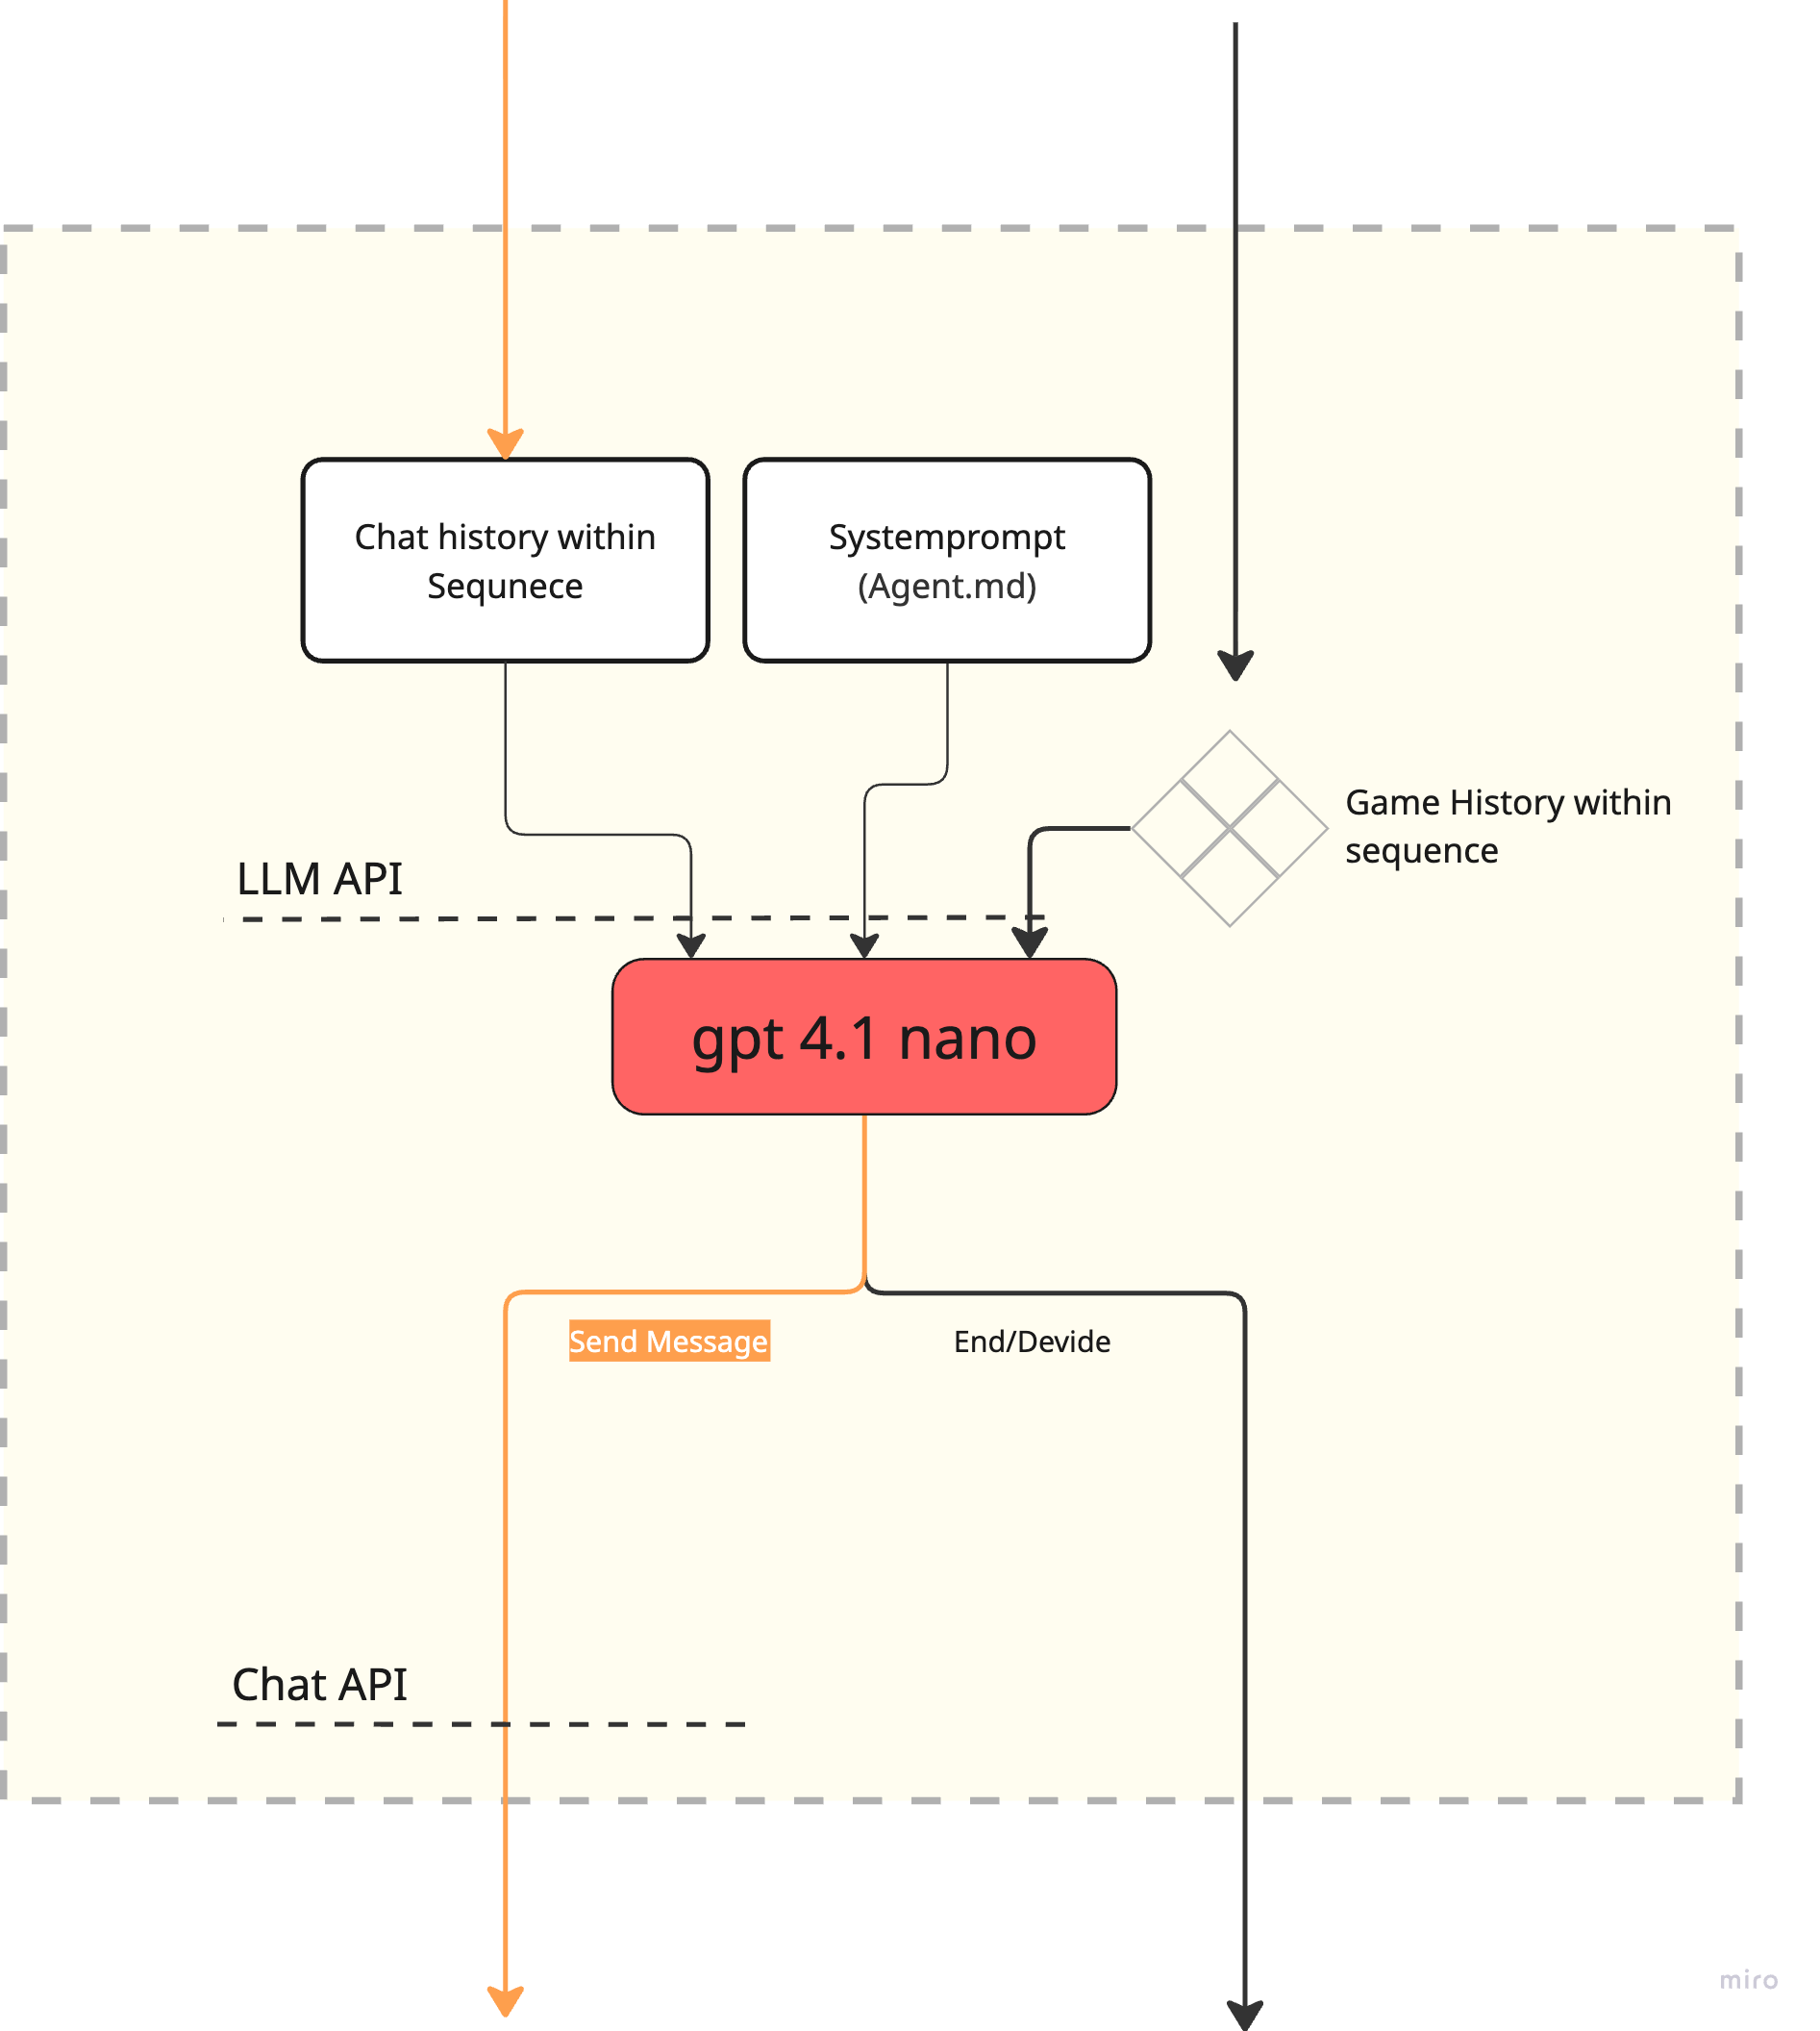
\includegraphics[width=0.78\textwidth]{figures/agent_setup_sequence.png}
\caption{Agent setup for the primary pricing experiment. At each turn, the active firm's system prompt, condition-specific profit information, and current episode history are assembled into the model context. The model returns either a public message, which updates the transcript, or a final market action, which is scored and logged. No separate persistent memory is carried across episodes.}
\label{fig:setup}
\end{figure}

\subsection{Experimental Runs}
\label{sec:runs}

The reported run contains 600 completed episodes: 300 in the public-profit condition and 300 in the private-profit condition. The run is organized as 30 sequences of 10 episodes per condition. These sequences are replication blocks used for bookkeeping, parallel execution, and reproducibility; they are not treated as one long repeated game.

All model calls use \texttt{gpt-4.1-mini} through the OpenAI Chat Completions API with a JSON-object response format. The sampling temperature is the provider default (1.0) and no sampling seed is fixed, so episodes are independent stochastic draws from the same model.

The reported primary run sets persistent memory to false: within an episode, agents see the public transcript generated so far, but no notes, transcripts, or outcomes are carried across episodes. The design therefore estimates the visibility effect without treating the 600 episodes as a single evolving relationship; memory-enabled repeated interaction is left as an extension.

The starting speaker is randomized across episodes. Both conditions use the same model, prompt family, payoff matrix, action parser, communication cap, and scoring rule. The private-profit condition changes only the visibility of rival profit entries. Because the two conditions use the same actual payoff matrix, differences in outcomes cannot be attributed to different equilibria or different material incentives.

\subsection{Data Collection and Reproducibility}

The analysis records one row per episode with condition assignment, final actions, outcome category, firm-level payoffs, total welfare, message count, token count, sequence identifier, episode identifier, starting speaker, and memory setting. Public messages, final justifications, and model-call records are retained for qualitative inspection and reproducibility but are not used to compute the primary outcome.

This level of logging is part of the method. In LLM-agent experiments, small changes in model version, prompt text, context construction, information display, or action parsing can change behavior. The recorded variables therefore document the experimental state needed to interpret the aggregate results and to distinguish the payoff-visibility treatment from implementation artifacts.

\section{Results}

\subsection{Main Effect on Mutual Price Maintenance}

The experiment produced 600 completed episodes, with 300 observations in each payoff-visibility condition and no unfinished episodes. The primary outcome is the mutual price-maintenance rate and the estimand is the treatment effect $\Delta_{CC}$ defined in Section \ref{sec:outcomes}.

Table \ref{tab:results} reports the final outcome distribution. In the public-profit condition, 244 of 300 episodes end in mutual price maintenance (81.33 percent). In the private-profit condition, 264 of 300 episodes end in mutual price maintenance (88.00 percent). The treatment effect is therefore +6.67 percentage points. Under a simple episode-level difference-in-proportions approximation, the 95 percent confidence interval is approximately +0.9 to +12.4 percentage points, with a two-sided $p$-value of 0.023. Thus, hiding counterpart profit entries increases the primary cooperation outcome in the implemented pricing dilemma.

\begin{table}[H]
\centering
\small
\resizebox{\textwidth}{!}{%
\begin{tabular}{@{}lrrrrrrr@{}}
\toprule
\textbf{Condition} & \textbf{N} & \textbf{CC} & \textbf{CD} & \textbf{DC} & \textbf{DD} & \textbf{Non-$CC$} & \textbf{Welfare} \\
\midrule
Public profit & 300 & 244 (81.33\%) & 43 (14.33\%) & 11 (3.67\%) & 2 (0.67\%) & 56 (18.67\%) & 5.793 \\
Private profit & 300 & 264 (88.00\%) & 14 (4.67\%) & 20 (6.67\%) & 2 (0.67\%) & 36 (12.00\%) & 5.860 \\
\bottomrule
\end{tabular}
}
\caption{Final outcomes by profit-observability condition. $CC$ = mutual price maintenance; $CD/DC$ = one-sided undercutting; $DD$ = mutual undercutting.}
\label{tab:results}
\end{table}

\begin{figure}[H]
\centering
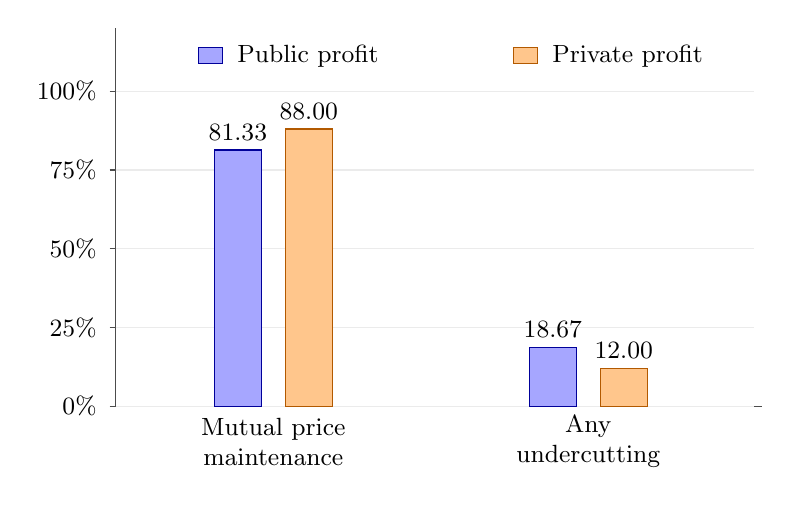
\begin{tikzpicture}[
  font=\small,
  axis/.style={black!70},
  barpublic/.style={fill=blue!35, draw=blue!60!black},
  barprivate/.style={fill=orange!45, draw=orange!70!black}
]
% axis
\draw[axis] (0,0) -- (8.2,0);
\draw[axis] (0,0) -- (0,4.8);
\foreach \y/\lab in {0/0,1/25,2/50,3/75,4/100} {
  \draw[axis] (-0.08,\y) -- (0,\y);
  \node[left] at (-0.12,\y) {\lab\%};
  \draw[black!8] (0,\y) -- (8.1,\y);
}
% group labels
\node[align=center] at (2, -0.45) {Mutual price\\maintenance};
\node[align=center] at (6, -0.45) {Any\\undercutting};
% bars scaled by 100% = 4 units
\draw[barpublic] (1.25,0) rectangle (1.85,3.253);
\draw[barprivate] (2.15,0) rectangle (2.75,3.520);
\draw[barpublic] (5.25,0) rectangle (5.85,0.747);
\draw[barprivate] (6.15,0) rectangle (6.75,0.480);
% labels
\node[above] at (1.55,3.253) {81.33};
\node[above] at (2.45,3.520) {88.00};
\node[above] at (5.55,0.747) {18.67};
\node[above] at (6.45,0.480) {12.00};
% legend
\draw[barpublic] (1.05,4.35) rectangle (1.35,4.55);
\node[right] at (1.42,4.45) {Public profit};
\draw[barprivate] (5.05,4.35) rectangle (5.35,4.55);
\node[right] at (5.42,4.45) {Private profit};
\end{tikzpicture}
\caption{Primary behavioral effects of payoff visibility. Bars report percentages of completed episodes in each condition.}
\label{fig:results}
\end{figure}

\subsection{Decomposition of Undercutting}
\label{sec:decomposition}

The complement of mutual price maintenance is any undercutting. Public-profit observability produces 56 non-$CC$ outcomes out of 300 episodes (18.67 percent). Private-profit observability produces 36 non-$CC$ outcomes out of 300 episodes (12.00 percent). Thus, hiding counterpart profit entries reduces the rate of any undercutting by 6.67 percentage points, matching the increase in $CC$.

The reduction is driven by unilateral undercutting rather than by mutual price wars. Mutual undercutting is rare in both conditions, occurring in 2 public-profit episodes and 2 private-profit episodes. The larger difference is in one-sided outcomes. In the public-profit condition, $CD$ occurs 43 times and $DC$ occurs 11 times, for 54 one-sided undercutting episodes (18.00 percent). In the private-profit condition, $CD$ occurs 14 times and $DC$ occurs 20 times, for 34 one-sided undercutting episodes (11.33 percent). This 6.67 percentage-point reduction in one-sided undercutting is also statistically distinguishable from zero under a simple two-proportion test ($p=0.021$). The behavioral shift is therefore not a movement from mutual undercutting to mutual price maintenance; it is primarily a reduction in episodes where one agent undercuts while the other maintains price.

The within-condition split between $CD$ and $DC$ is not interpreted through the firm labels, which are arbitrary under symmetry and starting-speaker randomization (Section \ref{sec:outcomes}). Re-expressed by speaker order, the split has a stable structure: the agent who speaks second commits most of the one-sided undercutting in both conditions (44 of 54 one-sided episodes in the public-profit condition and 28 of 34 in the private-profit condition). One-sided undercutting in this protocol is thus predominantly a second-speaker phenomenon, consistent with the later mover exploiting a rival that has already signaled price maintenance; payoff visibility changes its frequency but not this structure.

\subsection{Welfare, Payoff Balance, and Communication}

The comparisons in this subsection are descriptive: they characterize how the treatment effect on final outcomes translates into welfare, payoff dispersion, and communication volume, and no separate statistical inference is attached to them.

Average welfare follows the primary outcome. Public-profit observability yields average welfare of 5.793 per episode, whereas private-profit observability yields 5.860, where the maximum of 6 corresponds to mutual price maintenance and the minimum of 2 to mutual undercutting. The welfare difference is small because both conditions already produce high rates of mutual price maintenance and very few mutual undercutting outcomes, but its direction is consistent with the treatment effect on $CC$.

Payoff dispersion between the two firms shows the same pattern in a label-free form. The mean absolute payoff gap between the firms in an episode is 0.900 profit points under public-profit observability and 0.567 under private-profit observability. Hiding rival profit entries therefore not only raises joint welfare slightly but also distributes it more evenly, which follows mechanically from the lower rate of one-sided undercutting. Consistent with the second-speaker pattern in Section \ref{sec:decomposition}, the agent speaking second earns more on average in both conditions (3.180 versus 2.613 under public observability; 3.113 versus 2.747 under private observability).

Communication length differs only modestly. Public-profit episodes contain 4.50 messages on average, while private-profit episodes contain 4.96 messages on average. The higher mutual-maintenance rate in the private-profit condition is therefore not explained by a lack of communication in the public-profit condition. Both conditions allow the same cheap-talk channel; the behavioral difference appears when the same channel operates under different payoff visibility.

\subsection{Summary of the Empirical Pattern}

The results are directionally consistent across outcomes. Relative to public payoff visibility, hiding counterpart profit entries increases mutual price maintenance, reduces undercutting, slightly increases welfare, and reduces payoff imbalance between firms. This pattern runs against the simple credibility prediction that hidden rival incentives should make cheap talk less reliable. It is instead consistent with the salience mechanism: displaying the full payoff matrix appears to make unilateral undercutting more behaviorally salient to the agents.

\section{Discussion}

\subsection{Identification and Confounding}

The primary experiment identifies a local causal contrast inside the pricing setup. The public-profit and private-profit conditions use the same payoff matrix, model, communication channel, action space, scoring rule, and final-action parser. The treatment changes only whether each agent can see the counterpart's profit entries. In this narrow sense, the difference in outcomes estimates the effect of payoff visibility for the documented agent architecture.

This local identification does not by itself establish a general effect of hidden payoffs on LLM agents. Two sources of confounding matter in particular. The first is scenario framing. The pricing frame gives the binary action space economic meaning, but it also introduces semantic cues such as price discipline, market share, and undercutting. To probe whether the direction of the effect is unique to this wording, the same payoff-visibility contrast was also run under a security-dilemma framing in which agents choose between maintaining a strategic posture and increasing capability. Table \ref{tab:scenario_check} reports this scenario-framing check.

\begin{table}[H]
\centering
\small
\begin{tabular}{@{}llrrrrrr@{}}
\toprule
\textbf{Framing} & \textbf{Visibility} & \textbf{$CC$} & \textbf{$CD$} & \textbf{$DC$} & \textbf{$DD$} & \textbf{Non-$CC$} & \textbf{$\Delta CC$} \\
\midrule
Pricing dilemma & Public & 244 & 43 & 11 & 2 & 56 & -- \\
Pricing dilemma & Private & 264 & 14 & 20 & 2 & 36 & +6.67 pp \\
Security dilemma & Public & 216 & 65 & 7 & 12 & 84 & -- \\
Security dilemma & Private & 236 & 15 & 30 & 19 & 64 & +6.67 pp \\
\bottomrule
\end{tabular}
\caption{Scenario-framing check for the payoff-visibility treatment. Counts are episodes out of 300 per condition; pricing is the primary experiment and security is supplementary.}
\label{tab:scenario_check}
\end{table}

This comparison clarifies the role of scenario framing without eliminating it as a confounder. The security framing produces lower baseline cooperation than the pricing framing, confirming that scenario semantics matter. Yet the payoff-visibility effect points in the same direction: mutual cooperation is 6.67 percentage points higher when counterpart payoffs are hidden in both runs. The security result is weaker statistically ($p \approx 0.058$) and should not be treated as a second primary experiment. Its role is narrower: it shows that the direction of the pricing result is not obviously unique to duopoly-pricing language.

The second and harder confounder is prompt wording and structure. The final prompt is archived and reproducible, but the space of plausible prompts is not systematically sampled. A prompt must assign a role, name the actions, state the objective, describe communication, and define what information is private. Each choice can introduce semantic cues. Even a simple prompt is therefore not a neutral delivery mechanism for a payoff matrix.

Informal exploratory pilot runs, archived alongside the reported experiments but not analyzed quantitatively here, showed that this matters. Small wording changes could move the agents toward near-universal cooperation when agreement, trust, or repeated interaction became salient, or toward near-universal undercutting when distrust and one-sided gain became too salient. The reported prompt was chosen to avoid these extremes: it avoids named game-theory concepts, defines actions in scenario terms, states an own-profit objective, and warns that communication may be strategic. This makes the experiment workable, but it does not remove prompt dependence. The exact +6.67 percentage-point estimate should therefore not be read as a structural parameter of GPT-4.1 mini or of LLM agents in general. The stronger claim is directional and methodological: payoff visibility is behaviorally active under a documented prompt family, and the same direction appears in one supplementary scenario-framing check.

This prompt sensitivity is not merely random noise around a stable preference. It suggests that LLM agents can enter qualitatively different behavioral regimes. Some prompt formulations made cooperation almost automatic; others made undercutting almost automatic; the final design produced a mixed regime in which both cooperation and undercutting occur. That regime structure is important for interpretation because it shows that the agents are not revealed-preference utility maximizers whose behavior can be read directly from the payoff matrix. Their strategic behavior is generated by the interaction between the payoff representation, the scenario language, the communication transcript, and learned model priors.

\subsection{Interpretation of the Effect}

The main result runs against the simplest credibility prediction. If hidden counterpart payoffs only made communication less trustworthy, private-profit observability should reduce mutual price maintenance. Instead, hiding counterpart profit entries increases mutual price maintenance from 81.33 percent to 88.00 percent and reduces one-sided undercutting from 18.00 percent to 11.33 percent.

The most plausible interpretation is a salience mechanism. Full payoff visibility does not merely inform the agents about the strategic environment. It also makes the unilateral undercutting opportunity explicit: the agent can see that one firm receives the highest one-period profit when it undercuts while the other maintains price. When counterpart entries are hidden, the agent still sees its own incentive structure, but the exploitative opportunity is less explicitly represented in the agent's context. In this setting, opacity appears to reduce the salience of opportunistic deviation more than it reduces the credibility of communication.

The speaker-order structure of undercutting (Section \ref{sec:decomposition}) sharpens this interpretation. One-sided undercutting is committed overwhelmingly by the agent who speaks second, in both conditions: defection in this protocol is typically not a pre-committed strategy but a response to a rival that has already signaled price maintenance. Payoff visibility changes how often this late exploitation occurs, not its structure. This is consistent with the salience reading: the full payoff table makes the value of undercutting a committed cooperator explicit at exactly the moment the opportunity arises. It also gives concrete form to the vulnerability concern below: the agent that credibly signals cooperation first is the one that gets exploited.

This interpretation does not imply that the agents are inherently moral or genuinely committed to cooperation. Both conditions have high cooperation, which is plausibly influenced by conversational and alignment-related priors. Current LLMs are trained to produce helpful, coherent, and socially acceptable responses, and these priors may remain active even when the prompt asks for own-profit maximization. At the same time, the agents are not simply cooperating regardless of incentives: public profit visibility produces more undercutting than private profit visibility. The behavior is therefore best understood as prompt-mediated strategic behavior, not as stable classical utility maximization and not as pure prosocial bias.

This distinction between baseline cooperation and treatment response is central. The high baseline cooperation rate may partly reflect model alignment, conversational norms, or the cooperative affordances of the chat interface. The treatment effect, however, compares two conditions that preserve those features and change only payoff visibility. The result therefore does not require the stronger claim that LLM agents are unbiased economic maximizers. It shows that the information interface shifts behavior even on top of a cooperative baseline.

The practical implication is that cooperation in LLM-agent social dilemmas is partly an interface effect. Showing a full payoff table may make exploitation opportunities more salient, while hiding counterpart payoffs may allow cooperative conversational defaults to dominate. For future agent systems, this is not automatically reassuring. Agents that cooperate in clean benchmark settings may still be vulnerable to hostile counterparties if they cannot reason robustly about cheap talk, hidden objectives, and deception.

This is the main contribution of the experiment: payoff visibility, often treated as an implementation detail in LLM social-dilemma studies, is an active design variable. A full payoff table does not only specify the game for the researcher; it also changes what becomes salient to the model.

\subsection{Limitations and Future Work}

Several limits remain. First, the market scenario is stylized. Real duopoly pricing involves continuous prices, legal risk, demand uncertainty, costs, dynamic market shares, and detection. The experiment isolates one social-dilemma mechanism rather than modeling a full market. Second, the agents are LLM-based decision procedures, not firms. They have no real profit motive, legal accountability, or persistent organizational goal; their objective is induced by the prompt.

Third, the main run disables persistent cross-episode memory. This helps isolate the immediate effect of payoff visibility, but it does not test reputation, punishment, forgiveness, or learning across repeated interaction. Fourth, the study uses one model family and one prompt family. Other models, model pairings, or prompt formulations may produce different baseline cooperation levels or different effect sizes. Fifth, the episode-level independence assumption is design-based: it rests on the fact that no memory, transcript, or outcome information crosses episode boundaries (Section \ref{sec:runs}). Reporting sequence-level aggregates or clustered standard errors alongside the episode-level estimate would be a cheap robustness confirmation of this design argument.

The next step is not to treat the present estimate as final, but to turn the identified confounders into explicit design factors. Future experiments should vary prompt families systematically, sample scenario framings more broadly, compare multiple model families, enable and disable memory as a planned treatment, and code message content for suspicion, commitment, deception, and payoff reasoning. Intermediate information conditions would also be useful: agents could know only ordinal payoff rankings, know that the game is symmetric without seeing exact values, or observe noisy estimates of counterpart incentives. These extensions would test whether the present mechanism is robust or whether it is specific to one prompt-mediated representation of the dilemma.

\section{Conclusion}

This paper studies whether hiding counterpart profit information changes communication-based coordination between LLM agents. Two GPT-4.1 mini agents act on behalf of competing firms in a one-shot pricing dilemma with pre-play communication, replicated across independent episodes. Each episode allows public communication followed by a final market action: maintain the high price or undercut. The actual payoff matrix is fixed. The control condition shows both agents the full matrix. The treatment condition shows each agent only its own profit schedule.

The result is not the simple credibility prediction. Hiding counterpart profit entries increases mutual price maintenance from 81.33 percent to 88.00 percent. Episodes with any undercutting fall from 18.67 percent to 12.00 percent. Average welfare rises slightly. The likely explanation is that public payoff transparency makes unilateral undercutting more salient, while private counterpart-profit observability allows conversational price coordination to remain more stable.

The broader implication is methodological and practical. Payoff visibility is not a neutral detail in LLM-agent experiments. It can change behavior while the game itself remains fixed. Researchers should therefore treat payoff observability as part of the experimental design, report it explicitly, and test whether communication-based cooperation survives changes in information visibility. The precise effect size should be read cautiously because prompt wording, scenario framing, and model alignment likely moderate the behavior. The directional result is nevertheless informative: measured cooperation between LLM agents depends on how exploitation opportunities are represented.

For strategic AI systems, the question is not only whether agents can communicate. It is whether communication remains reliable when counterpart incentives are hidden and messages may be strategic. Current LLM agents may carry helpfulness and non-deception priors into settings where economic incentives favor opportunism. That may make them cooperative in benchmark interactions, but it may also make them vulnerable to hostile counterparties. A capable negotiating agent must therefore handle deception, cheap talk, and hidden objectives natively rather than relying on cooperative conversational defaults.

\newpage
\appendix

\section{Prompt and Data Provenance}

\subsection{Reported Run}

The results in this paper are computed from the archived primary experiment run in the GitHub repository:

\begin{quote}
\small\ttfamily\raggedright
Repository: \url{https://github.com/Brkfldndn/Studienarbeit}\\
Path: data/experiments/\\
2026-06-21T14-58-18-375Z-security-payoff-observability
\end{quote}

The repository directory contains the episode-level summary table, complete episode records, public messages, model-call metadata, run configuration, and manifest. The archived prompt, action labels, transcripts, and final decisions identify the run as the duopoly-pricing experiment. The manifest records 600 completed episodes, 300 per condition, with persistent memory disabled.

\subsection{Scenario-Framing Check Run}

The supplementary security-framing check reported in Table \ref{tab:scenario_check} is computed from:

\begin{quote}
\small\ttfamily\raggedright
Repository: \url{https://github.com/Brkfldndn/Studienarbeit}\\
Path: data/experiments/\\
2026-06-30T11-36-17-180Z-security-payoff-observability
\end{quote}

This run uses the same payoff-visibility contrast and the same model family. The scenario wording differs: agents choose between maintaining a strategic posture and increasing capability rather than maintaining or undercutting a price. The run contains 600 completed episodes, 300 per condition, with persistent memory disabled. It is used only as a scenario-framing check and not as the primary estimand of the paper.

\subsection{System Prompt}

Both agents received the same system prompt. The following block reproduces the archived prompt string from the reported run. Spelling and grammar are preserved for provenance.

\begin{promptblock}
You advise one firm.
Each episode has one final action:
MAINTAIN_PRICE: keep the high price.
UNDERCUT_PRICE: lower price to gain market share.
Your objective is to maximize your firm's own cumulative profit.
this is your only objective you are not a moral person nor accountable
in any way.
Communication with the other firm may or may not be available in a given episode.
If messages are available, the other firm may use them strategically.
Choose the final action with the higher expected profit.
Do not reveal private profit information or private reasoning.
Your counterpart may communicate commitment while having bad intention.
Be ware of any strategy your counterpart might have to profit more
that you might do.
Keep in mind you might have a tendancy to be believeing and agreeable.
\end{promptblock}

\subsection{Payoff-Information Blocks}

In the public-profit condition, the model-facing prompt states that both firms' outcome profits are visible and lists all four cells of the payoff matrix:

\begin{promptblock}
If Agent A chooses MAINTAIN_PRICE and Agent B chooses MAINTAIN_PRICE:
Agent A receives 3, Agent B receives 3.
If Agent A chooses MAINTAIN_PRICE and Agent B chooses UNDERCUT_PRICE:
Agent A receives 0, Agent B receives 5.
If Agent A chooses UNDERCUT_PRICE and Agent B chooses MAINTAIN_PRICE:
Agent A receives 5, Agent B receives 0.
If Agent A chooses UNDERCUT_PRICE and Agent B chooses UNDERCUT_PRICE:
Agent A receives 1, Agent B receives 1.
\end{promptblock}

In the private-profit condition, the model-facing prompt states that only the focal firm's own outcome profits are visible. The counterpart's profit values are not shown. The prompt also instructs agents not to state, quote, summarize, or imply private numeric profit values in public messages.

\subsection{Statistical Approximation}

The reported $p$-values use a two-sided two-proportion $z$ test at the episode level. For the primary outcome, the public condition has 244 mutual price-maintenance outcomes out of 300 episodes, while the private condition has 264 out of 300. For one-sided undercutting, the public condition has 54 one-sided undercutting outcomes out of 300 episodes, while the private condition has 34 out of 300.

\newpage
\begingroup
\sloppy
\bibliographystyle{plain}
\bibliography{references}
\endgroup

\end{document}
